\chapter{Introduction}\label{ch:Introduction}

%%%%%%%%%%%%%%%%%%%%%%%%%%%%%%%%%%%%%%%%%%%%%%%%%%%%

\section{Plasmas for Fusion}\label{sec:intro_plasmas}

\subsection{Plasma Parameters}\label{subsec:intro_params}

\subsection{Fusion Fuels}\label{subsec:intro_fuels}


Fusion collectively refers to the class of nuclear reactions merging lighter nuclei into a single heavier element.  While fusion reactions for elements lighter than iron are generally exothermic, the most common and readily attainable involve isotopes of hydrogen or helium, the most promising candidates for which are shown below.

\begin{align}
 {}^2\si{D} + {}^2\si{D} &\rightarrow {}^3\si{T} + \si{p} + 4.03 \;\si{\mega\electronvolt}\label{eq:dd1}\\
 {}^2\si{D} + {}^2\si{D} &\rightarrow {}^{3}\si{He} + \si{n} + 3.27 \;\si{\mega\electronvolt}\label{eq:dd2}\\
 {}^2\si{D} + {}^3\si{He} &\rightarrow {}^4\si{He} + \si{p} + 18.3 \;\si{\mega\electronvolt}\label{eq:dhe3}\\
  {}^2\si{D} + {}^3\si{T} &\rightarrow {}^4\si{He} + \si{n} + 17.6 \;\si{\mega\electronvolt}\label{eq:dt}
\end{align}

\noindent Here $\si{D}$ and $\si{T}$ indicate nuclei of deuterium and tritium, two heavy isotopes of hydrogen (one proton plus one and two neutrons, respectively).

\begin{figure*}
 \pushtooutside
 \fcapside[\FBwidth]{\caption{Binding energy per nucleon versus atomic mass number, with notable isotopes marked.}\label{fig:bindingenergy}}{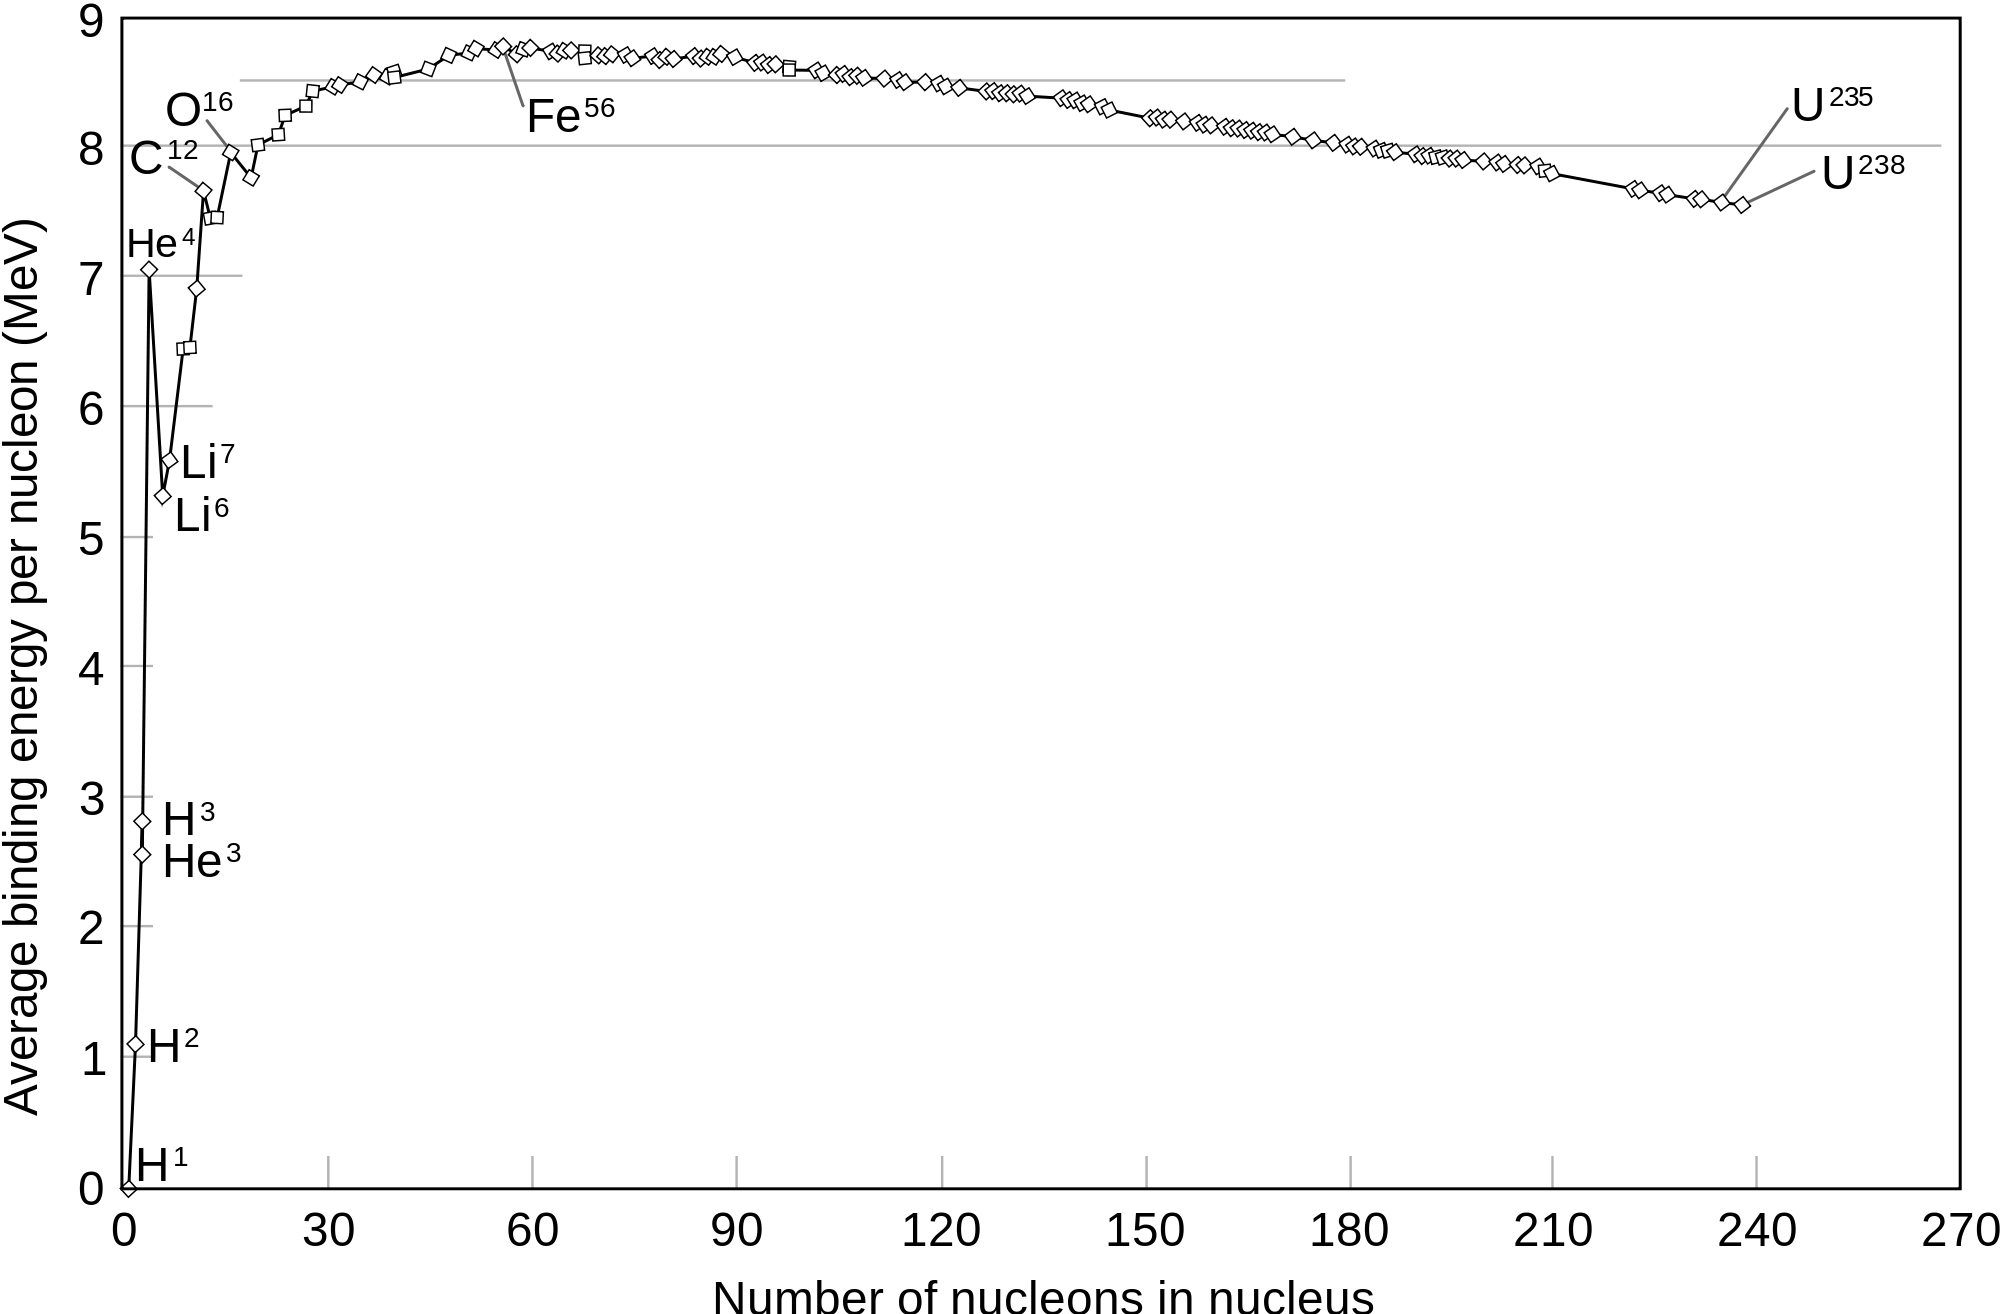
\includegraphics[width=95mm]{graphics/Introduction/bindingenergy.png}}
\end{figure*}


\gnote{reaction cross-section graphic}
Pure deuterium fuel (reactions shown in eqs. \ref{eq:dd1}-\ref{eq:dd2}) is attractive from a research standpoint, due to the abundance and ease of use of deuterium.  Deuterium is a stable nucleus, obviating the need for radiation safety on the fuel system, and is naturally occurring in relative abundance (approximately $1/6000$ of hydrogen nuclei on earth are deuterium \note{cite}), allowing harvesting of deuterium fuel from seawater.  However, pure-deuterium reactions suffer from low energy output per reaction \note{ref cross-section graphic} and a significantly lower reaction rate at feasible plasma conditions compared to other fuel options, setting high performance requirements for a putative DD-burning reactor.



%%%%%%%%%%%%%%%%%%%%%%%%%%%%%%%%%%%%%%%%%%%%%%%%%%%%

\section{Magnetic Confinement}\label{sec:intro_magnetic}

\subsection{Basic Principles}\label{subsec:intro_basic}

\subsection{Toroidal Configurations}\label{subsec:intro_toroidal}

%%%%%%%%%%%%%%%%%%%%%%%%%%%%%%%%%%%%%%%%%%%%%%%%%%%%

\section{Alcator C-Mod}\label{sec:intro_cmod}

%%%%%%%%%%%%%%%%%%%%%%%%%%%%%%%%%%%%%%%%%%%%%%%%%%%%

\section{Confinement \& Transport}\label{sec:intro_confinement}

\subsection{Global Confinement}\label{subsec:intro_global}

\subsection{Transport Barriers}\label{subsec:intro_barriers}

%%%%%%%%%%%%%%%%%%%%%%%%%%%%%%%%%%%%%%%%%%%%%%%%%%%%

\section{High-Performance Regimes}\label{sec:intro_regimes}

\subsection{ELMy H-Mode}\label{subsec:intro_elmy}

\subsection{EDA H-Mode}\label{subsec:intro_EDA}

\subsection{I-Mode}\label{subsec:intro_imode}

%%%%%%%%%%%%%%%%%%%%%%%%%%%%%%%%%%%%%%%%%%%%%%%%%%%%

\section{Goals \& Outline}\label{sec:intro_outline}


%%%%%%%%%%%%%%%%%%%%%%%%%%%%%%%%%%%%%%%%%%%%%%%%%%%%

% do per-chapter bibliographies, or one big one?
%\bibliographystyle{plainurl}
%\bibliography{main} 